% Options for packages loaded elsewhere
\PassOptionsToPackage{unicode}{hyperref}
\PassOptionsToPackage{hyphens}{url}
%
\documentclass[
]{book}
\usepackage{amsmath,amssymb}
\usepackage{lmodern}
\usepackage{iftex}
\ifPDFTeX
  \usepackage[T1]{fontenc}
  \usepackage[utf8]{inputenc}
  \usepackage{textcomp} % provide euro and other symbols
\else % if luatex or xetex
  \usepackage{unicode-math}
  \defaultfontfeatures{Scale=MatchLowercase}
  \defaultfontfeatures[\rmfamily]{Ligatures=TeX,Scale=1}
\fi
% Use upquote if available, for straight quotes in verbatim environments
\IfFileExists{upquote.sty}{\usepackage{upquote}}{}
\IfFileExists{microtype.sty}{% use microtype if available
  \usepackage[]{microtype}
  \UseMicrotypeSet[protrusion]{basicmath} % disable protrusion for tt fonts
}{}
\makeatletter
\@ifundefined{KOMAClassName}{% if non-KOMA class
  \IfFileExists{parskip.sty}{%
    \usepackage{parskip}
  }{% else
    \setlength{\parindent}{0pt}
    \setlength{\parskip}{6pt plus 2pt minus 1pt}}
}{% if KOMA class
  \KOMAoptions{parskip=half}}
\makeatother
\usepackage{xcolor}
\IfFileExists{xurl.sty}{\usepackage{xurl}}{} % add URL line breaks if available
\IfFileExists{bookmark.sty}{\usepackage{bookmark}}{\usepackage{hyperref}}
\hypersetup{
  pdftitle={Course Outline: Time Series Data in R},
  pdfauthor={Harrison Brown},
  hidelinks,
  pdfcreator={LaTeX via pandoc}}
\urlstyle{same} % disable monospaced font for URLs
\usepackage{color}
\usepackage{fancyvrb}
\newcommand{\VerbBar}{|}
\newcommand{\VERB}{\Verb[commandchars=\\\{\}]}
\DefineVerbatimEnvironment{Highlighting}{Verbatim}{commandchars=\\\{\}}
% Add ',fontsize=\small' for more characters per line
\usepackage{framed}
\definecolor{shadecolor}{RGB}{248,248,248}
\newenvironment{Shaded}{\begin{snugshade}}{\end{snugshade}}
\newcommand{\AlertTok}[1]{\textcolor[rgb]{0.94,0.16,0.16}{#1}}
\newcommand{\AnnotationTok}[1]{\textcolor[rgb]{0.56,0.35,0.01}{\textbf{\textit{#1}}}}
\newcommand{\AttributeTok}[1]{\textcolor[rgb]{0.77,0.63,0.00}{#1}}
\newcommand{\BaseNTok}[1]{\textcolor[rgb]{0.00,0.00,0.81}{#1}}
\newcommand{\BuiltInTok}[1]{#1}
\newcommand{\CharTok}[1]{\textcolor[rgb]{0.31,0.60,0.02}{#1}}
\newcommand{\CommentTok}[1]{\textcolor[rgb]{0.56,0.35,0.01}{\textit{#1}}}
\newcommand{\CommentVarTok}[1]{\textcolor[rgb]{0.56,0.35,0.01}{\textbf{\textit{#1}}}}
\newcommand{\ConstantTok}[1]{\textcolor[rgb]{0.00,0.00,0.00}{#1}}
\newcommand{\ControlFlowTok}[1]{\textcolor[rgb]{0.13,0.29,0.53}{\textbf{#1}}}
\newcommand{\DataTypeTok}[1]{\textcolor[rgb]{0.13,0.29,0.53}{#1}}
\newcommand{\DecValTok}[1]{\textcolor[rgb]{0.00,0.00,0.81}{#1}}
\newcommand{\DocumentationTok}[1]{\textcolor[rgb]{0.56,0.35,0.01}{\textbf{\textit{#1}}}}
\newcommand{\ErrorTok}[1]{\textcolor[rgb]{0.64,0.00,0.00}{\textbf{#1}}}
\newcommand{\ExtensionTok}[1]{#1}
\newcommand{\FloatTok}[1]{\textcolor[rgb]{0.00,0.00,0.81}{#1}}
\newcommand{\FunctionTok}[1]{\textcolor[rgb]{0.00,0.00,0.00}{#1}}
\newcommand{\ImportTok}[1]{#1}
\newcommand{\InformationTok}[1]{\textcolor[rgb]{0.56,0.35,0.01}{\textbf{\textit{#1}}}}
\newcommand{\KeywordTok}[1]{\textcolor[rgb]{0.13,0.29,0.53}{\textbf{#1}}}
\newcommand{\NormalTok}[1]{#1}
\newcommand{\OperatorTok}[1]{\textcolor[rgb]{0.81,0.36,0.00}{\textbf{#1}}}
\newcommand{\OtherTok}[1]{\textcolor[rgb]{0.56,0.35,0.01}{#1}}
\newcommand{\PreprocessorTok}[1]{\textcolor[rgb]{0.56,0.35,0.01}{\textit{#1}}}
\newcommand{\RegionMarkerTok}[1]{#1}
\newcommand{\SpecialCharTok}[1]{\textcolor[rgb]{0.00,0.00,0.00}{#1}}
\newcommand{\SpecialStringTok}[1]{\textcolor[rgb]{0.31,0.60,0.02}{#1}}
\newcommand{\StringTok}[1]{\textcolor[rgb]{0.31,0.60,0.02}{#1}}
\newcommand{\VariableTok}[1]{\textcolor[rgb]{0.00,0.00,0.00}{#1}}
\newcommand{\VerbatimStringTok}[1]{\textcolor[rgb]{0.31,0.60,0.02}{#1}}
\newcommand{\WarningTok}[1]{\textcolor[rgb]{0.56,0.35,0.01}{\textbf{\textit{#1}}}}
\usepackage{longtable,booktabs,array}
\usepackage{calc} % for calculating minipage widths
% Correct order of tables after \paragraph or \subparagraph
\usepackage{etoolbox}
\makeatletter
\patchcmd\longtable{\par}{\if@noskipsec\mbox{}\fi\par}{}{}
\makeatother
% Allow footnotes in longtable head/foot
\IfFileExists{footnotehyper.sty}{\usepackage{footnotehyper}}{\usepackage{footnote}}
\makesavenoteenv{longtable}
\usepackage{graphicx}
\makeatletter
\def\maxwidth{\ifdim\Gin@nat@width>\linewidth\linewidth\else\Gin@nat@width\fi}
\def\maxheight{\ifdim\Gin@nat@height>\textheight\textheight\else\Gin@nat@height\fi}
\makeatother
% Scale images if necessary, so that they will not overflow the page
% margins by default, and it is still possible to overwrite the defaults
% using explicit options in \includegraphics[width, height, ...]{}
\setkeys{Gin}{width=\maxwidth,height=\maxheight,keepaspectratio}
% Set default figure placement to htbp
\makeatletter
\def\fps@figure{htbp}
\makeatother
\setlength{\emergencystretch}{3em} % prevent overfull lines
\providecommand{\tightlist}{%
  \setlength{\itemsep}{0pt}\setlength{\parskip}{0pt}}
\setcounter{secnumdepth}{5}
\usepackage{booktabs}
\ifLuaTeX
  \usepackage{selnolig}  % disable illegal ligatures
\fi
\usepackage[]{natbib}
\bibliographystyle{plainnat}

\title{Course Outline: Time Series Data in R}
\author{Harrison Brown}
\date{2022-06-05}

\begin{document}
\maketitle

{
\setcounter{tocdepth}{1}
\tableofcontents
}
\hypertarget{welcome}{%
\chapter*{Welcome}\label{welcome}}
\addcontentsline{toc}{chapter}{Welcome}

Welcome to the course outline for \emph{Time Series Data in R}! This course offers methods and workflows for analyzing and interpreting time series data, an overview of when, why, and how to use time series data, and various utilities and packages in R that are beneficial to analysts.

\hypertarget{course-outline-manipulating-time-series-data-in-r}{%
\chapter*{Course Outline: Manipulating Time Series Data in R}\label{course-outline-manipulating-time-series-data-in-r}}
\addcontentsline{toc}{chapter}{Course Outline: Manipulating Time Series Data in R}

\emph{This course will introduce learners to working with time series data in R. Learners will explore how to store and format data in date and time objects as well as how to manipulate time series datasets through subsetting, indexing, and extraction. Examples of time series data across a variety of fields in business and science should be discussed. The course will cover summarization, frequency, missing data, resampling, and comparison techniques as well as window functions for both rolling and expanding windows.}

Packages Used:

\begin{itemize}
\tightlist
\item
  \texttt{base} and \texttt{stats} (default libraries, but I wanted to name them explicitly)
\item
  \texttt{zoo}
\item
  \texttt{lubridate} (so far, only for the \texttt{lubridate::year()} function (Lesson 3.3). I wanted to keep the package dependencies to just \texttt{zoo}, but \texttt{lubridate::year()} makes the conversion in Lesson 3.3 much easier for the learner).
\end{itemize}

Terms Defined:

\begin{itemize}
\tightlist
\item
  \emph{Temporal Data}: Data that describe a measurement of a variable at a specific point in time, such as the chance of rain on June 20, 2009, or the price of a particular stock market at 2:00 p.m. on January 9, 1987.
\item
  \emph{Temporal Attributes}: The characteristics and attributes that define the sampling frequency (\emph{monthly}, \emph{weekly}, etc.) and the start- and end-points of \emph{Temporal Data}.
\item
  \emph{Core Data}: Within R, \emph{Core Data} is the ``measured'' data without any temporal information; i.e., the set of values that do not have any temporal attributes.
\item
  \emph{Imputing}: The statistical process of substituting missing values through a certain process, e.g.~replacing missing values with 0 or the average of adjacent values.
\end{itemize}

Functions are written in \texttt{code\ text} below each \textbf{Learning Objective}

\hypertarget{chapter-1-introduction-to-time-series-data}{%
\section*{Chapter 1: Introduction to Time Series Data}\label{chapter-1-introduction-to-time-series-data}}
\addcontentsline{toc}{section}{Chapter 1: Introduction to Time Series Data}

\hypertarget{lesson-1.1-what-is-time-series-data}{%
\subsection*{\texorpdfstring{Lesson 1.1: \emph{What is Time Series Data}}{Lesson 1.1: What is Time Series Data}}\label{lesson-1.1-what-is-time-series-data}}
\addcontentsline{toc}{subsection}{Lesson 1.1: \emph{What is Time Series Data}}

\begin{itemize}
\tightlist
\item
  \textbf{Learning Objective:} Learner will be able to understand the core principal of time series data: time series analysis studies \emph{how} a variable changes with time, rather than just analyzing the variable at different points in time.
\item
  \textbf{Learning Objective:} Learners will be introduced to basic exploratory functions to examine and visualize time series objects in R:

  \begin{itemize}
  \tightlist
  \item
    \texttt{print()} (specifically, \texttt{print.ts()})
  \item
    \texttt{plot()} (specifically, \texttt{plot.ts()})
  \end{itemize}
\end{itemize}

\hypertarget{lesson-1.2-temporal-data-classes-in-r}{%
\subsection*{\texorpdfstring{Lesson 1.2: \emph{Temporal data classes in R}}{Lesson 1.2: Temporal data classes in R}}\label{lesson-1.2-temporal-data-classes-in-r}}
\addcontentsline{toc}{subsection}{Lesson 1.2: \emph{Temporal data classes in R}}

\begin{itemize}
\tightlist
\item
  \textbf{Learning Objective:} Learner will be introduced to different formats for temporal data in R, such as the \texttt{Date}, \texttt{numeric}, and \texttt{character} classes:
\item
  e.g.: 2022-01-30, \texttt{19022}, and ``2022-01-30'' share the same information, but in different formats
\item
  \textbf{Learning Objective:} Learners will be able to coerce objects of different classes to the desired class, and check the classes of objects:

  \begin{itemize}
  \tightlist
  \item
    \texttt{class()}
  \item
    \texttt{as.Date()}
  \item
    \texttt{as.numeric()}
  \item
    \texttt{as.character()}
  \end{itemize}
\end{itemize}

\hypertarget{lesson-1.3-formatting-dates-in-r}{%
\subsection*{\texorpdfstring{Lesson 1.3: \emph{Formatting \texttt{Date}s in R}}{Lesson 1.3: Formatting Dates in R}}\label{lesson-1.3-formatting-dates-in-r}}
\addcontentsline{toc}{subsection}{Lesson 1.3: \emph{Formatting \texttt{Date}s in R}}

\begin{itemize}
\tightlist
\item
  \textbf{Learning Objective:} Learners will be introduced to formatting Dates in R by manipulating character and Date vectors, in order to both improve legibility of and standardize the format of temporal data.

  \begin{itemize}
  \tightlist
  \item
    \texttt{format()} (specifically, \texttt{format.Date()})

    \begin{itemize}
    \tightlist
    \item
      e.g.: \texttt{format(as.Date("1987-04-12"),\ "\%b\ \%d,\ \%Y")} gives \texttt{"May\ 12,\ 1987"}
    \end{itemize}
  \end{itemize}
\end{itemize}

\hypertarget{chapter-2-time-series-objects-in-r}{%
\section*{Chapter 2: Time Series objects in R}\label{chapter-2-time-series-objects-in-r}}
\addcontentsline{toc}{section}{Chapter 2: Time Series objects in R}

\hypertarget{lesson-2.1-time-series-attributes}{%
\subsection{\texorpdfstring{Lesson 2.1: \emph{Time Series Attributes}}{Lesson 2.1: Time Series Attributes}}\label{lesson-2.1-time-series-attributes}}

\begin{itemize}
\tightlist
\item
  \textbf{Learning Objective:} Learners will be able to retrieve the temporal attributes (start and end points, as well as frequency) of a time series object:

  \begin{itemize}
  \tightlist
  \item
    \texttt{start()}
  \item
    \texttt{end()}
  \item
    \texttt{frequency()}
  \end{itemize}
\end{itemize}

\hypertarget{lesson-2.2-create-a-time-series-object-in-base-r}{%
\subsection*{\texorpdfstring{Lesson 2.2: \emph{Create a Time Series object in Base R}}{Lesson 2.2: Create a Time Series object in Base R}}\label{lesson-2.2-create-a-time-series-object-in-base-r}}
\addcontentsline{toc}{subsection}{Lesson 2.2: \emph{Create a Time Series object in Base R}}

\begin{itemize}
\tightlist
\item
  \textbf{Learning Objective:} Learners will convert a vector of observations with a known start time and frequency (e.g., monthly data starting in the year 2004) into a \texttt{ts} object. By adding temporal attributes to the data, such as start time, frequency, and end time, learners will be able to properly manipulate data with the methods outlined in the remainder of the course.

  \begin{itemize}
  \tightlist
  \item
    \texttt{ts()}
  \item
    \texttt{as.ts()}
  \item
    e.g.: assume \texttt{data} is a numeric vector of observations; \texttt{ts(data,\ start\ =\ zoo::as.yearmon("Jan\ 2004"),\ frequency\ =\ 12)}
  \end{itemize}
\end{itemize}

\hypertarget{lesson-2.3-using-the-zoo-package-to-store-time-series-data}{%
\subsection*{\texorpdfstring{Lesson 2.3: \emph{Using the Zoo Package to store time series data}}{Lesson 2.3: Using the Zoo Package to store time series data}}\label{lesson-2.3-using-the-zoo-package-to-store-time-series-data}}
\addcontentsline{toc}{subsection}{Lesson 2.3: \emph{Using the Zoo Package to store time series data}}

\begin{itemize}
\tightlist
\item
  \textbf{Learning Objective:} Learners will be introduced to the \texttt{zoo} object from the \texttt{zoo} package, and why is it different from base \texttt{ts}:

  \begin{itemize}
  \tightlist
  \item
    Zoo can use irregular time intervals, more robust, etc.
  \end{itemize}
\item
  \textbf{Learning Objective:} Learners will be able to convert and coerce time series objects with the \texttt{zoo} package:

  \begin{itemize}
  \tightlist
  \item
    \texttt{zoo::zoo()}
  \item
    \texttt{zoo::as.zoo()}
  \end{itemize}
\end{itemize}

\hypertarget{lesson-2.4-using-zoo-to-extract-time-and-data-vectors}{%
\subsection*{\texorpdfstring{Lesson 2.4: \emph{Using Zoo to extract time and data vectors}}{Lesson 2.4: Using Zoo to extract time and data vectors}}\label{lesson-2.4-using-zoo-to-extract-time-and-data-vectors}}
\addcontentsline{toc}{subsection}{Lesson 2.4: \emph{Using Zoo to extract time and data vectors}}

\begin{itemize}
\tightlist
\item
  \textbf{Learning Objective:} Learners can extract ``core data'' and time data from a \texttt{ts} or \texttt{zoo} object:

  \begin{itemize}
  \tightlist
  \item
    \texttt{time()}
  \item
    \texttt{zoo::coredata()}
  \end{itemize}
\end{itemize}

\hypertarget{chapter-3-subsetting-extracting-and-resampling}{%
\section*{Chapter 3: Subsetting, Extracting, and Resampling}\label{chapter-3-subsetting-extracting-and-resampling}}
\addcontentsline{toc}{section}{Chapter 3: Subsetting, Extracting, and Resampling}

\hypertarget{lesson-3.1-subsetting-a-window-of-observations}{%
\subsection*{\texorpdfstring{Lesson 3.1: \emph{Subsetting a window of observations}}{Lesson 3.1: Subsetting a window of observations}}\label{lesson-3.1-subsetting-a-window-of-observations}}
\addcontentsline{toc}{subsection}{Lesson 3.1: \emph{Subsetting a window of observations}}

\begin{itemize}
\tightlist
\item
  \textbf{Learning Objective:} Learners will be able to extract a window of observations between a set of given points in time:

  \begin{itemize}
  \tightlist
  \item
    \texttt{window()}

    \begin{itemize}
    \tightlist
    \item
      \texttt{window(data,\ start\ =\ "2020-01-01",\ end\ =\ "2020-12-31")} retrieves observations between (inclusive) Jan 1, 2020 and Dec 31, 2020.
    \end{itemize}
  \item
    \texttt{as.Date()}

    \begin{itemize}
    \tightlist
    \item
      The \texttt{window} function can usually coerce the \texttt{start} and \texttt{end} arguments correctly, but it's good practice to tell the function exactly the date and format we want to use.
    \end{itemize}
  \end{itemize}
\end{itemize}

\hypertarget{lesson-3.2-subsetting-specific-observations}{%
\subsection*{\texorpdfstring{Lesson 3.2: \emph{Subsetting specific observations}}{Lesson 3.2: Subsetting specific observations}}\label{lesson-3.2-subsetting-specific-observations}}
\addcontentsline{toc}{subsection}{Lesson 3.2: \emph{Subsetting specific observations}}

\begin{itemize}
\tightlist
\item
  \textbf{Learning Objective:} Learners will use the \texttt{\textquotesingle{}{[}\textquotesingle{}} operator with \texttt{as.Date()} to extract an observation from a specific time or a specific index:

  \begin{itemize}
  \tightlist
  \item
    \texttt{\textquotesingle{}{[}\textquotesingle{}}

    \begin{itemize}
    \tightlist
    \item
      \texttt{data{[}1:20{]}} retrieves observations 1 through 20; \texttt{data{[}12{]}} retrieves the 12\textsuperscript{th} observation, etc.
    \end{itemize}
  \item
    \texttt{as.Date()}

    \begin{itemize}
    \tightlist
    \item
      \texttt{data{[}as.Date("2020-03-01"){]}} retrieves the observation for March 1, 2020.
    \end{itemize}
  \item
    \texttt{zoo::as.yearmon()}

    \begin{itemize}
    \tightlist
    \item
      If data are stored in year-month format, \texttt{data{[}as.yearmon("Jul\ 2019"){]}} retrieves the observation for the month of July, 2019.
    \end{itemize}
  \end{itemize}
\end{itemize}

\hypertarget{lesson-3.3-resampling-observations}{%
\subsection*{\texorpdfstring{Lesson 3.3: \emph{Resampling observations}}{Lesson 3.3: Resampling observations}}\label{lesson-3.3-resampling-observations}}
\addcontentsline{toc}{subsection}{Lesson 3.3: \emph{Resampling observations}}

\begin{itemize}
\tightlist
\item
  \textbf{Learning Objective:} Learner will be able to re-sample observations to any interval of time (yearly, monthly, quarterly, etc.):

  \begin{itemize}
  \tightlist
  \item
    \texttt{aggregate()} (specifically, \texttt{aggregate.zoo()} for \texttt{zoo} objects)
  \item
    \texttt{lubridate::year()}
  \item
    \texttt{zoo::yearqtr()}
  \item
    \texttt{zoo::yearmon()}

    \begin{itemize}
    \tightlist
    \item
      e.g.: \texttt{aggregate(data,\ by\ =\ lubridate::year,\ FUN\ =\ sum)} finds sums of observations within each year.
    \end{itemize}
  \end{itemize}
\end{itemize}

\hypertarget{lesson-3.4-imputing-missing-values}{%
\subsection*{\texorpdfstring{Lesson 3.4: \emph{Imputing Missing Values}}{Lesson 3.4: Imputing Missing Values}}\label{lesson-3.4-imputing-missing-values}}
\addcontentsline{toc}{subsection}{Lesson 3.4: \emph{Imputing Missing Values}}

\begin{itemize}
\tightlist
\item
  \textbf{Learning Objective:} Learners will use the \texttt{zoo} package to impute missing values with either linear interpolation or cubic spline interpolation:

  \begin{itemize}
  \tightlist
  \item
    \texttt{zoo::na.approx()} and \texttt{zoo::na.spline()}, respectively
  \item
    \texttt{zoo::fill()} can be used to fill all \texttt{NA} values with a given value, e.g.~0.
  \end{itemize}
\end{itemize}

\hypertarget{chapter-4-rolling-and-expanding-windows}{%
\section*{Chapter 4: Rolling and Expanding Windows}\label{chapter-4-rolling-and-expanding-windows}}
\addcontentsline{toc}{section}{Chapter 4: Rolling and Expanding Windows}

\hypertarget{lesson-4.1-what-are-windows}{%
\subsection*{\texorpdfstring{Lesson 4.1: \emph{What are windows?}}{Lesson 4.1: What are windows?}}\label{lesson-4.1-what-are-windows}}
\addcontentsline{toc}{subsection}{Lesson 4.1: \emph{What are windows?}}

\begin{itemize}
\tightlist
\item
  \textbf{Learning Objective:} Learners will understand the utility of rolling and expanding windows: finding moving averages, cumulative sums, etc.
\item
  \textbf{Learning Objective:} Learners will be able to perform a rolling window operation on a time series, creating a moving average (or moving sum) of an arbitrary length:

  \begin{itemize}
  \tightlist
  \item
    \texttt{zoo::rollapply()}
  \item
    \texttt{zoo::rollapplyr()} (convenience wrapper for \texttt{zoo::rollapply(align\ =\ "right")})

    \begin{itemize}
    \tightlist
    \item
      e.g.: \texttt{zoo::rollapplyr(daily\_data,\ FUN\ =\ mean,\ width\ =\ 7)} to create a 7-day rolling average from \texttt{daily\_data}
    \end{itemize}
  \end{itemize}
\end{itemize}

\hypertarget{lesson-4.2-calculating-an-expanding-window}{%
\subsection*{\texorpdfstring{Lesson 4.2: \emph{Calculating an Expanding Window}}{Lesson 4.2: Calculating an Expanding Window}}\label{lesson-4.2-calculating-an-expanding-window}}
\addcontentsline{toc}{subsection}{Lesson 4.2: \emph{Calculating an Expanding Window}}

\begin{itemize}
\tightlist
\item
  \textbf{Learning Objective:} Learners will be able to create an expanding window -- a rolling window where the ``start'' is fixed and the ``end'' moves:

  \begin{itemize}
  \tightlist
  \item
    \texttt{cumsum()}
  \item
    \texttt{seq\_along()}

    \begin{itemize}
    \tightlist
    \item
      \texttt{cumsum(data)\ /\ seq\_along(data)} gives a rolling mean, which exists in \texttt{dplyr::cummean()} but not base R.
    \end{itemize}
  \end{itemize}
\end{itemize}

\hypertarget{lesson-4.3-zoos-roll-functions}{%
\subsection*{\texorpdfstring{Lesson 4.3: \emph{zoo's roll functions}}{Lesson 4.3: zoo's roll functions}}\label{lesson-4.3-zoos-roll-functions}}
\addcontentsline{toc}{subsection}{Lesson 4.3: \emph{zoo's roll functions}}

\begin{itemize}
\item
  \textbf{Learning Objective:} Learners will be introduced to the other \texttt{roll*} functions within \texttt{zoo}, allowing for more compact and legible code when performing rolling window calculations:

  \begin{itemize}
  \item
    \texttt{zoo::rollmean()}
  \item
    \texttt{zoo::rollmedian()}
  \item
    \texttt{zoo::rollsum()}
  \item
    \texttt{zoo::rollmax()}
  \end{itemize}
\end{itemize}

\hypertarget{lesson-4.4-plotting-windows-alongside-data}{%
\subsection*{\texorpdfstring{Lesson 4.4: \emph{Plotting windows alongside Data}}{Lesson 4.4: Plotting windows alongside Data}}\label{lesson-4.4-plotting-windows-alongside-data}}
\addcontentsline{toc}{subsection}{Lesson 4.4: \emph{Plotting windows alongside Data}}

\begin{itemize}
\tightlist
\item
  \textbf{Learning Objective:} Learners will be able to plot the rolling/expanding window alongside the original data, in order to visually assess how these operations affect the data:

  \begin{itemize}
  \tightlist
  \item
    \texttt{plot()}
  \item
    \texttt{lines()}
  \end{itemize}
\end{itemize}

\hypertarget{capstone-exercise}{%
\chapter{Capstone Exercise}\label{capstone-exercise}}

The final exercise for this course involves performing a time series analysis on real-world data: Carbon Dioxide concentration at the Mauna Loa Observatory, from early 1959 to Present. You'll go through the process of importing the data, converting to a time series object (with \texttt{zoo}), imputing missing values, and plotting the resulting data. Additionally, you will create an aggregate of the data, as well as a rolling window average of the data.

\hypertarget{importing-the-data}{%
\section{Importing the Data}\label{importing-the-data}}

\begin{Shaded}
\begin{Highlighting}[]
\CommentTok{\# The following libraries are included for you}

\FunctionTok{library}\NormalTok{(zoo)}
\CommentTok{\# Sample data from the Mauna Loa Observatory}
\CommentTok{\# https://gml.noaa.gov/webdata/ccgg/trends/co2/co2\_mm\_mlo.csv}

\CommentTok{\# Data is already pre{-}processed as a \textasciigrave{}zoo\textasciigrave{} object. It contains missing values,}
\CommentTok{\# so we\textquotesingle{}ll need to impute those!}

\CommentTok{\# This will be hidden from the users, of course.}
\NormalTok{missing\_co2 }\OtherTok{\textless{}{-}} \FunctionTok{readRDS}\NormalTok{(}\StringTok{"data/missing.Rds"}\NormalTok{)}
\end{Highlighting}
\end{Shaded}

\newpage

\hypertarget{visualizing-the-data}{%
\section{Visualizing the Data}\label{visualizing-the-data}}

Perform basic data exploration by:

\begin{enumerate}
\def\labelenumi{\arabic{enumi}.}
\tightlist
\item
  Printing the first 20 observations with \texttt{head()}, and,
\item
  Creating a plot of the data with \texttt{plot()}
\end{enumerate}

\begin{Shaded}
\begin{Highlighting}[]
\FunctionTok{head}\NormalTok{(missing\_co2, }\AttributeTok{n =} \DecValTok{20}\NormalTok{)}
\end{Highlighting}
\end{Shaded}

\begin{verbatim}
## Jan 1959 Feb 1959 Mar 1959 Apr 1959 May 1959 Jun 1959 Jul 1959 Aug 1959 
##   315.58   316.48   316.65   317.72   318.29   318.15       NA       NA 
## Sep 1959 Oct 1959 Nov 1959 Dec 1959 Jan 1960 Feb 1960 Mar 1960 Apr 1960 
##   313.84   313.33   314.81       NA   316.43   316.98       NA       NA 
## May 1960 Jun 1960 Jul 1960 Aug 1960 
##   320.04   319.59   318.18   315.90
\end{verbatim}

\begin{Shaded}
\begin{Highlighting}[]
\FunctionTok{plot}\NormalTok{(missing\_co2)}
\end{Highlighting}
\end{Shaded}

\begin{center}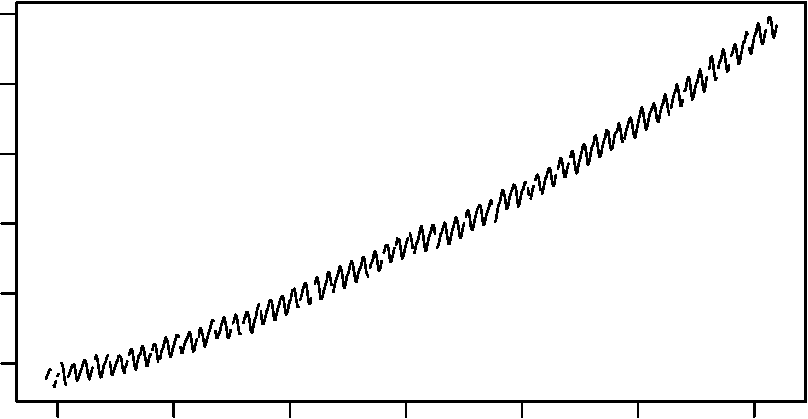
\includegraphics{timeseries_files/figure-latex/q1-2-1} \end{center}

Notice that there are ``holes'' in the data? this suggests that we've got NA values, which is apparent when we view the first few observations with \texttt{head()}.

\newpage

\hypertarget{imputing-the-missing-values}{%
\section{Imputing the Missing Values}\label{imputing-the-missing-values}}

Impute the missing values with a \emph{cubic spline} interpolation, then plot the results

\begin{Shaded}
\begin{Highlighting}[]
\NormalTok{filled\_co2 }\OtherTok{\textless{}{-}} \FunctionTok{na.spline}\NormalTok{(missing\_co2)}
\end{Highlighting}
\end{Shaded}

\begin{Shaded}
\begin{Highlighting}[]
\FunctionTok{plot}\NormalTok{(filled\_co2)}
\end{Highlighting}
\end{Shaded}

\begin{center}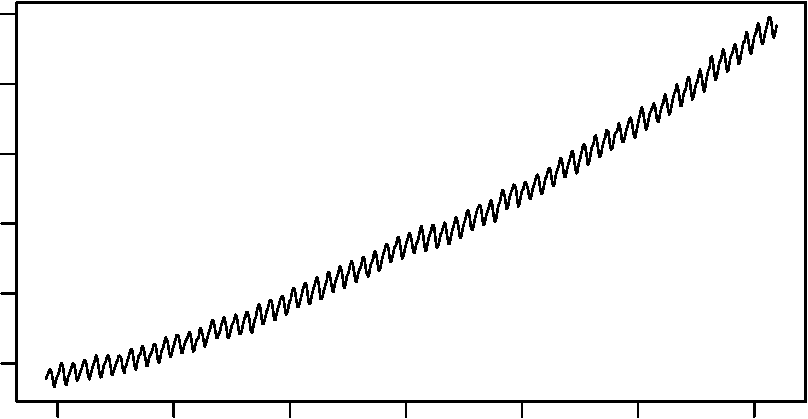
\includegraphics{timeseries_files/figure-latex/q2-2-1} \end{center}

\newpage

\hypertarget{yearly-aggregate}{%
\section{Yearly Aggregate}\label{yearly-aggregate}}

Using \texttt{aggregate()}, create a yearly mean of the data, then plot the data

*Hint: use \texttt{lubridate::year()}

\begin{Shaded}
\begin{Highlighting}[]
\NormalTok{yearly\_co2 }\OtherTok{\textless{}{-}} \FunctionTok{aggregate}\NormalTok{(filled\_co2,}
  \AttributeTok{by =}\NormalTok{ lubridate}\SpecialCharTok{::}\NormalTok{year,}
  \AttributeTok{FUN =}\NormalTok{ mean}
\NormalTok{)}


\FunctionTok{plot}\NormalTok{(yearly\_co2)}
\end{Highlighting}
\end{Shaded}

\begin{center}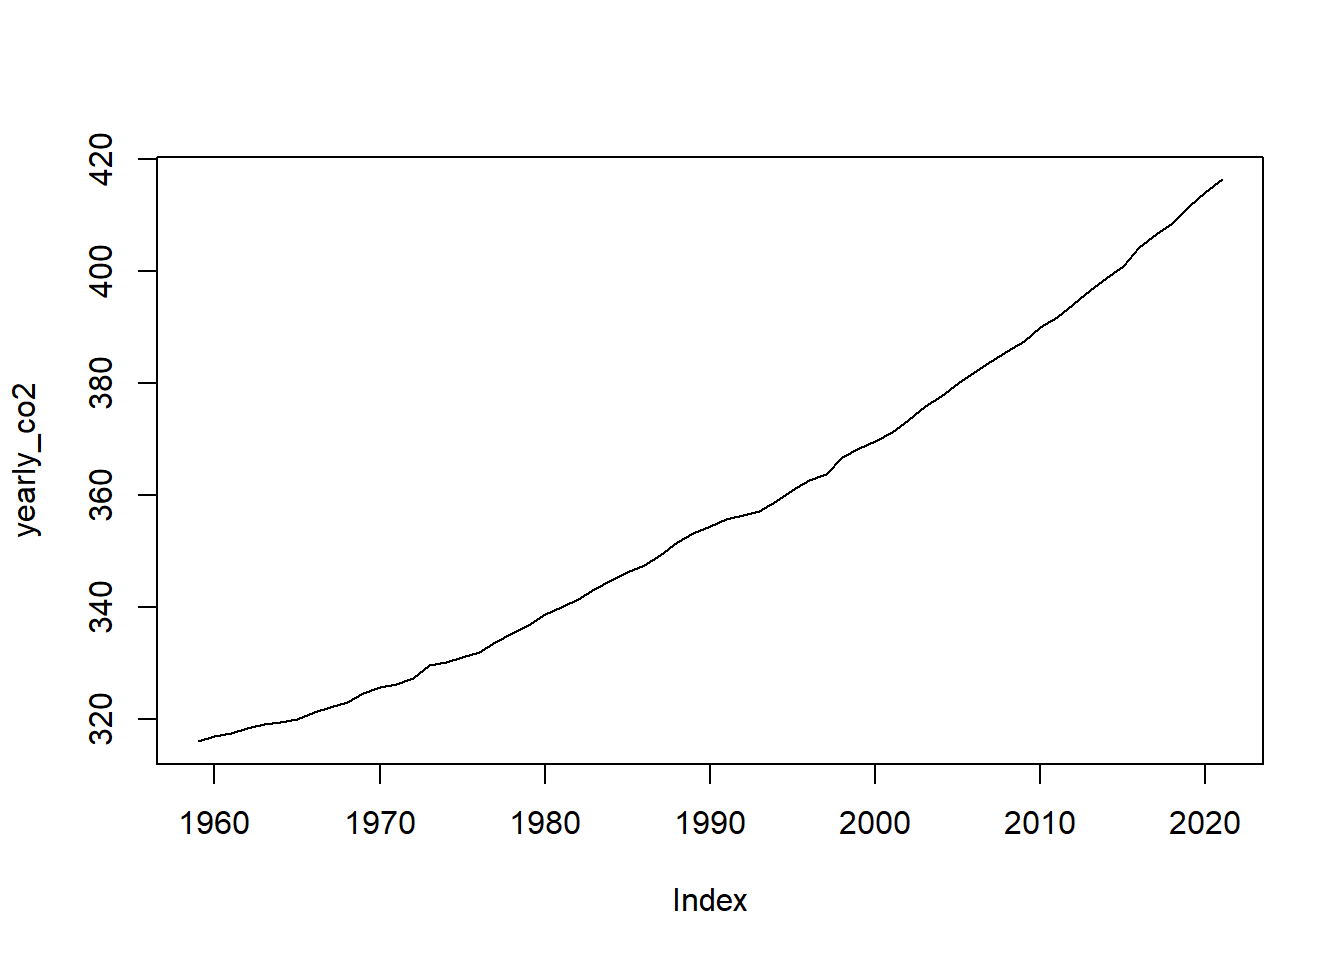
\includegraphics{timeseries_files/figure-latex/q3-1-1} \end{center}

\newpage

\hypertarget{rolling-window}{%
\section{Rolling Window}\label{rolling-window}}

Calculate a 12-month rolling window average of the data, then overlay the results (in blue) on top of the original data. Label the x-axis as ``Time'' and the y-axis as ``CO2 Concentration'', and give your graph the title ``Monthly CO2 Concentration at Mauna Loa Observatory''

\begin{Shaded}
\begin{Highlighting}[]
\NormalTok{roll }\OtherTok{\textless{}{-}} \FunctionTok{rollapplyr}\NormalTok{(filled\_co2,}
  \AttributeTok{FUN =}\NormalTok{ mean,}
  \AttributeTok{width =} \DecValTok{12}
\NormalTok{)}

\FunctionTok{plot}\NormalTok{(filled\_co2,}
     \AttributeTok{xlab =} \StringTok{"Time"}\NormalTok{,}
     \AttributeTok{ylab =} \StringTok{"CO2 Concentration"}\NormalTok{,}
     \AttributeTok{main =} \StringTok{"CO2 Concentration at Mauna Loa Observatory"}\NormalTok{)}

\FunctionTok{lines}\NormalTok{(roll, }\AttributeTok{col =} \StringTok{"blue"}\NormalTok{)}
\end{Highlighting}
\end{Shaded}

\begin{center}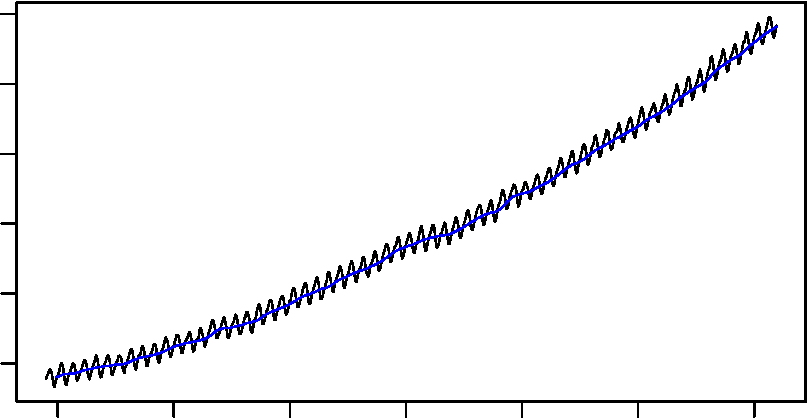
\includegraphics{timeseries_files/figure-latex/q4-1} \end{center}

\newpage

\hypertarget{given-code}{%
\section{Given Code}\label{given-code}}

The following code is given to the learners at the beginning of the exercise:

\begin{Shaded}
\begin{Highlighting}[]
\CommentTok{\# Question 1: Explore the Data}
\FunctionTok{\_\_\_}\NormalTok{(missing\_co2, }\AttributeTok{\_\_\_ =}\NormalTok{ \_\_\_)}

\FunctionTok{\_\_\_}\NormalTok{(missing\_co2)}
\end{Highlighting}
\end{Shaded}

\begin{Shaded}
\begin{Highlighting}[]
\CommentTok{\# Question 2: Impute Missing Values}

\NormalTok{filled\_co2 }\OtherTok{\textless{}{-}} \FunctionTok{\_\_\_}\NormalTok{(\_\_\_)}

\FunctionTok{\_\_\_}\NormalTok{(filled\_co2)}
\end{Highlighting}
\end{Shaded}

\begin{Shaded}
\begin{Highlighting}[]
\CommentTok{\# Question 3: Find Yearly Mean Aggregate}
\NormalTok{yearly\_co2 }\OtherTok{=} \FunctionTok{aggregate}\NormalTok{(\_\_\_, }\AttributeTok{by =}\NormalTok{ \_\_\_, }\AttributeTok{FUN =}\NormalTok{ \_\_\_)}

\FunctionTok{\_\_\_}\NormalTok{(\_\_\_)}
\end{Highlighting}
\end{Shaded}

\begin{Shaded}
\begin{Highlighting}[]
\CommentTok{\# Question 4: Calculate a Rolling Window}
\NormalTok{roll }\OtherTok{\textless{}{-}} \FunctionTok{rollapplyr}\NormalTok{(filled\_co2, }\AttributeTok{FUN =}\NormalTok{ \_\_\_, }\AttributeTok{width =} \DecValTok{12}\NormalTok{)}

\FunctionTok{plot}\NormalTok{(\_\_\_,}
     \AttributeTok{xlab =}\NormalTok{ \_\_\_,}
     \AttributeTok{ylab =}\NormalTok{ \_\_\_,}
     \AttributeTok{main =} \StringTok{"CO2 Concentration at Mauna Loa Observatory"}\NormalTok{)}

\FunctionTok{lines}\NormalTok{(\_\_\_, }\AttributeTok{col =}\NormalTok{ \_\_\_)}
\end{Highlighting}
\end{Shaded}


  \bibliography{book.bib,packages.bib}

\end{document}
